% THIS IS SIGPROC-SP.TEX - VERSION 3.1
% WORKS WITH V3.2SP OF ACM_PROC_ARTICLE-SP.CLS
% APRIL 2009
%
% It is an example file showing how to use the 'acm_proc_article-sp.cls' V3.2SP
% LaTeX2e document class file for Conference Proceedings submissions.
% ----------------------------------------------------------------------------------------------------------------
% This .tex file (and associated .cls V3.2SP) *DOES NOT* produce:
%       1) The Permission Statement
%       2) The Conference (location) Info information
%       3) The Copyright Line with ACM data
%       4) Page numbering
% ---------------------------------------------------------------------------------------------------------------
% It is an example which *does* use the .bib file (from which the .bbl file
% is produced).
% REMEMBER HOWEVER: After having produced the .bbl file,
% and prior to final submission,
% you need to 'insert'  your .bbl file into your source .tex file so as to provide
% ONE 'self-contained' source file.
%
% Questions regarding SIGS should be sent to
% Adrienne Griscti ---> griscti@acm.org
%
% Questions/suggestions regarding the guidelines, .tex and .cls files, etc. to
% Gerald Murray ---> murray@hq.acm.org
%
% For tracking purposes - this is V3.1SP - APRIL 2009

\documentclass{acm_proc_article-sp}

\usepackage{graphics}
\begin{document}

%\title{The Coloured Petri Nets Modeling Languages for Concurrent Systems}

\title{Coloured Petri Nets: A Graphical Language for Formal Modeling and Validation of Concurrent Systems}
\subtitle{}

%\titlenote{A full version of this paper is available as
%\textit{Author's Guide to Preparing ACM SIG Proceedings Using
%\LaTeX$2_\epsilon$\ and BibTeX} at
%\texttt{www.acm.org/eaddress.htm}}}
%
% You need the command \numberofauthors to handle the 'placement
% and alignment' of the authors beneath the title.
%
% For aesthetic reasons, we recommend 'three authors at a time'
% i.e. three 'name/affiliation blocks' be placed beneath the title.
%
% NOTE: You are NOT restricted in how many 'rows' of
% "name/affiliations" may appear. We just ask that you restrict
% the number of 'columns' to three.
%
% Because of the available 'opening page real-estate'
% we ask you to refrain from putting more than six authors
% (two rows with three columns) beneath the article title.
% More than six makes the first-page appear very cluttered indeed.
%
% Use the \alignauthor commands to handle the names
% and affiliations for an 'aesthetic maximum' of six authors.
% Add names, affiliations, addresses for
% the seventh etc. author(s) as the argument for the
% \additionalauthors command.
% These 'additional authors' will be output/set for you
% without further effort on your part as the last section in
% the body of your article BEFORE References or any Appendices.

\numberofauthors{2} %  in this sample file, there are a *total*
% of EIGHT authors. SIX appear on the 'first-page' (for formatting
% reasons) and the remaining two appear in the \additionalauthors section.
%
\author{
% You can go ahead and credit any number of authors here,
% e.g. one 'row of three' or two rows (consisting of one row of three
% and a second row of one, two or three).
%
% The command \alignauthor (no curly braces needed) should
% precede each author name, affiliation/snail-mail address and
% e-mail address. Additionally, tag each line of
% affiliation/address with \affaddr, and tag the
% e-mail address with \email.
%
% 1st. author
\alignauthor
Kurt Jensen\\
       \affaddr{Computer Science Department}\\
       \affaddr{Aarhus University, Denmark}\\
       \email{kjensen@cs.au.dk}
% 2nd. author
\alignauthor
Lars M. Kristensen\\
       \affaddr{Department of Computing}\\
       \affaddr{Bergen University College, Norway}\\
       \email{lmkr@hib.no}
}

\maketitle
\begin{abstract}

Coloured Petri Nets (CPNs) combine Petri nets with a programming
language to obtain a scalable formal modeling language for concurrent
systems. Petri nets provide the formal foundation for modeling
concurrency and synchronization, and a programming language provides
the primitives for modeling data manipulation and creating compact and
parameterizable models. We provide an example driven introduction to
the core syntactical and semantical constructs of the CPN modeling
language, and briefly surveys how quantitative and qualitative
behavioral properties of CPN models can be validated using
simulation-based performance analysis and explicit state space
exploration. In addition, we give a brief overview of CPN Tools which
provide tool support for the practical use of CPNs, and provide
pointers to some significant examples where the CPN technology has
been put into practical use in an industrial setting. As we proceed,
we provide a historical perspective on the research that led to the
development of the CPN language.

\end{abstract}

% A category with the (minimum) three required fields
\category{H.4}{Information Systems Applications}{Miscellaneous}
%A category including the fourth, optional field follows...
\category{D.2.8}{Software Engineering}{Metrics}[complexity measures, performance measures]

\terms{Theory}

\keywords{TODO} % NOT required for Proceedings

\newcommand{\com}[1]{
        \mbox{}
       \marginpar{\hrule\footnotesize\raggedright\hspace{0pt}#1\vspace{2mm}}
}

\newcommand{\todo}[1]{
       TODO: \mbox{}
       \marginpar{\hrule\footnotesize\raggedright\hspace{0pt}#1\vspace{2mm}}
}

\newcommand\concept[1]{{\em #1}}
\newcommand\figitem[1]{{\sf #1}}
\newcommand\smlcode[1]{{\tt{#1}}}
\newcommand\ignore[1]{}
\newcommand\fix[1]{\textbf{#1}?}


\section{Introduction}

The vast majority of IT systems today can be characterized as
concurrent and distributed systems in that their operation inherently
relies on communication, synchronization, and resource sharing between
concurrently executing software components and applications. This is a
development that has been accelerated first with the pervasive
presence of the Internet as a communication infrastructure, and in
recent years by, e.g, cloud- and web-based services, mobile
applications, and multi-core computing architectures.

% main motivation and application domain of CPNs

The development of Colored Petri Nets (CPNs) was initiated in the
early 80'es when distributed systems were becoming a major paradigm
for future computing systems. The goal of the CPN modeling language
was to develop a formally founded modeling language for concurrent
systems that would make it possible to formally analyze and validate
concurrent systems, and which from a modeling perspective would scale
to industrial systems. A main motivation behind the research into CPNs
(and many other formal modeling languages) was that the engineering of
correct concurrent systems is a challenging task due to their complex
behavior which may result in subtle bugs if not carefully designed. As
concurrent systems are becoming still more pervasive and critical to
society, formal techniques for concurrent systems were -- and still are
-- a highly relevant technology to support the engineering of reliable
concurrent systems. Many formal modelling languages for concurrent
systems have been developed, and examples of widely used languages
include Statecharts \cite{statecharts}, Timed Automata
\cite{timedautomata}, and Promela \cite{promela}.

% historical perspectic on development and roots

At their origin, CPNs build on Petri nets (see Sidebar~I on Petri nets),
which were introduced by Carl Adam Petri in his doctoral thesis
published in 1962 \cite{capetri:thesis} as a formalism for concurrency
and synchronization. The introduction of Petri nets by C.A. Petri was
far ahead of the time where distributed systems were invented and
computers started to have parallel processes. At that time, programs
and processing were considered to be sequential and
deterministic. Hence, it was extremely visionary of C.A. Petri to
predict the importance of being able to understand and characterize
the basic concepts of concurrency. In Petri nets, concurrency is a
fundamental concept in that Petri nets are inherently based on the idea
that behavior is (implicitly) concurrent unless explicitly
synchronized. This is in contrast to many other modeling formalisms
where concurrency must be explicitly introduced using parallel
composition operators. A further advantage of Petri nets is that they
rely on very few basic concepts, and are still able to model a wide
range of communication and synchronization concepts and patterns.\\

\vspace*{-1.5em}
%\noindent\rule{\columnwidth}{0.2em}
\paragraph*{\textsc{\textbf{SIDEBAR I: Petri nets}}}
A Petri net in its basic form is called a Place/Transition net (PTN) and
is a directed bi-partite graph with nodes consisting of places (drawn
as ellipses) and transitions (drawn as rectangles). The state of a
Petri net is called a marking and consists of a distribution of tokens
(drawn as black dots) positioned on the places. The execution of a
Petri net (also referred to as the token game) consists of occurrences
of enabled transitions removing tokens from input places and adding
tokens to output places as described by integer arc weights thereby
changing the current state (marking) of the Petri net. An abundance of
structural analysis methods (e.g., invariants and net reductions) as
well as dynamic analysis methods (e.g., state spaces and coverability
graphs) exists for Petri nets \cite{girault}\hfill$\qed$ \\
%\noindent\rule{\columnwidth}{0.2em}
% disadvantages - need for further development

In the decade following the introduction by C.~A. Petri, Petri nets
were widely accepted as one of the most well-founded theories to
describe important behavioral concepts such as concurrency, conflict
(non-determinism), synchronization, and resource sharing. Petri nets
were also used to model and analyze smaller concurrent
systems. However, the practical use soon revealed a serious
shortcoming. Petri nets (in their basic form) do not scale to large
systems unless one models the systems at a very high level of
abstraction. The primary reasons for this is that Petri nets are not
well-suited for modeling systems in which data and manipulation of
data plays a crucial role. Furthermore, Petri nets did not provide
concepts that made it easy to scale models according to some system
parameter, e.g., increase the number of servers in a modeled system
without having to make major changes to the model. This implied that
the use of Petri nets for practical modelling was decelerating. To
remedy this situation many researchers proposed different ad-hoc
extensions to Petri nets. This created a large variety of different
Petri net modeling languages. Many ad-hoc extensions were not
well-defined, and even when they were, they often had fundamental
theoretical problems. Whenever a new ad-hoc extension was introduced,
all the basic concepts and analysis methods had to be redefined -- to
apply for the extended Petri net language (with the ad-hoc
extension). With the invention of the first (text-based) computer
tools to support the analysis of Petri net models, the situation
became acute. Whenever a new ad-hoc extension was introduced (to
handle a modeling shortcoming) all existing computer tools became
void, and could only be used after time-consuming and error-prone
reprogramming. Hence, there was an urgent need to develop a class of
Petri nets that were general enough to handle a large variety of
different application areas without the need of making ad-hoc
extensions.

The first successful step towards a common more powerful class of
Petri nets were taken by Genrich and Lautenbach in 1979 with the
introduction of Predicate/Transition Nets (PrT nets)
\cite{genrich:81}. Their work was inspired by earlier work on
transition nets with \concept{colored tokens} by Schiffers and Wedde
\cite{schiffers:78} and transition nets with \concept{complex
  conditions} by Shapiro \cite{shapiro:78}. The basic idea behind PrT
nets was to introduce a set of colored tokens which can be
distinguished from each other -- in contrast to the indistinguishable
black tokens in basic Petri nets. In this way it became possible to
model different processes in a single subnet. PrT nets used arc
expressions to define how transitions can occur in different ways
(occurrence modes) depending on the colors of the involved input and
output tokens. The invention of colored distinguishable tokens in PrT
nets was a significant step forward -- but it still had some
limitations. PrT nets only had one set of token colors, and all places
had to use this set (or Cartesian products based on this set).

The second step towards a more general class of Petri nets was taken
by Jensen in his PhD thesis in 1980 with the introduction of the first
kind of Colored Petri Nets (CPNs) \cite{jensen:81}. This Petri net
model allowed the modeler to use a number of different color
sets. This made it possible to represent data values in a more
intuitive way instead of having to encode all data into a single
shared set. It later turned out to be convenient to define the color
sets by means of data types known from programming languages, such as
products, records, lists, and enumerations. The use of types had three
implications: Token colors became structured (and hence much more
powerful); type checking became possible (making it much easier to
locate modeling errors); and color sets, arc expressions and guards
could be specified by the well-known and powerful syntax and semantics
known from programming languages. This gave the modeler a convenient
way to handle complex data and specify the often complex interaction
between data and system behavior. A third step forward was taken by
Huber, Jensen, and Shapiro in 1990 with the introduction of
Hierarchical CPNs \cite{huber:91}. Their work was heavily inspired by
the hierarchy concepts in the Structured Analysis and Design Technique
(SADT) developed by Marca and McGowan \cite{sadt}. It was Shapiro who
got the idea to port the SADT hierarchy concepts to CPNs.  The
introduction of hierarchical CPNs allowed the modeler to structure a
large CPN model into a number of interacting and re-usable modules --
in a similar way as known from programming languages. This implied
that Petri net models of large systems become much more tractable,
since they can be split into modules of a reasonable size and the
model can be viewed at different levels of abstraction.


\ignore{
The shortcoming of ordinary Petri nets outlined above prompted a
research direction into the development of high-level Petri nets which
... KURT TO ADD HISTORICAL PERSPECTIVE ON THE DEVELOPMENT OF
HIGH-LEVEL NETS. WE NEED TO TALK ABOUT STANDARD ML SOMEWHERE AND SAY
THAT CPN ML IS BASED ON SML.
}


\section{Coloured Petri Nets}
\label{sect:language}

% modules - substitution transitions

To give an informal introduction to the concepts of CPNs, we use a CPN
model of a distributed two-phase commit transaction system.\footnote{The CPN model presented in this paper is available via \texttt{http://X.Y.Z/cpncommitmodel}}.  The reader
interested in the formal definition of CPNs is referred to
\cite{newcpnbook}. The CPN model of the two-phase commit system is
comprised of four \concept{modules} hierarchically organized into
three levels. Figure~\ref{fig:commit} shows the top-level module which
consists of two \concept{substitution transitions} (drawn as
rectangles with double-lined borders) representing the
\figitem{Coordinator} and the \figitem{Workers} in the system. Each of
the substitution transitions has an associated \concept{submodule}
that model the detailed behavior of the coordinator and the workers,
respectively. The name of the submodule is written in the rectangular
tag positioned at the bottom of each substitution transition.

\begin{figure}[b]
\centering
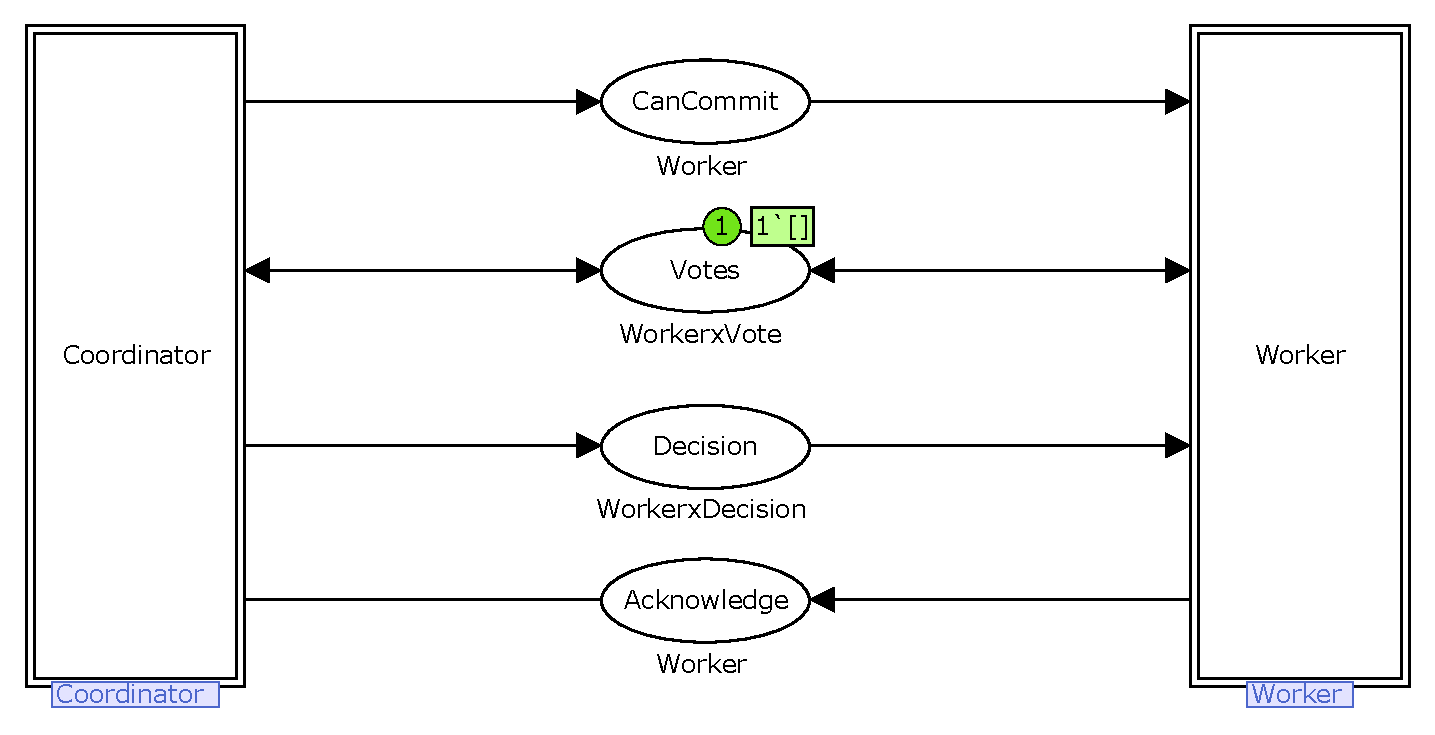
\includegraphics[scale=.5]{figures/Commit.eps}
\caption{The top-level module of the CPN model.}
\label{fig:commit}
\end{figure}

% places - tokens - colours - and colour sets

The two substitution transitions are connected via directed
\concept{arcs} to the four places \figitem{CanCommit},
\figitem{Votes}, \figitem{Decision}, and \figitem{Acknowledge} (drawn
as ellipses). Places connected to substitution transitions are called
\concept{socket places} and are linked to \concept{port} places on the
associated submodules (to be presented shortly). The coordinator and
the workers interact by producing and consuming \concept{tokens} on
the places. These tokens carry data values and the type of tokens that
may reside on a place is determined by the \concept{type} of the place
(written in text below the place). For historical reasons the types of
places are called \concept{color sets}. Figure~\ref{fig:coloursets}
lists the definitions of the color sets used for the four places in
Fig.~\ref{fig:commit}. These color sets are defined using the CPN ML
programming language which is based on the functional language
Standard ML \cite{sml}.

The \smlcode{Worker} color set is an indexed type consisting of the
values \smlcode{wrk(1),wrk(2),...,wrk(W)} used to model the identity
of the worker processes. The symbolic constant \smlcode{W} is used to
specify the number of worker processes considered. The color set
\smlcode{Vote} is an enumeration type containing the values
\smlcode{Yes} and \smlcode{No}, and is used to model that a worker may
vote \smlcode{Yes} or \smlcode{No} to commit the transaction. The
color set \smlcode{WorkerxVote} is a product type containing pairs
consisting of a worker and its vote. The color set \smlcode{Decision}
is an enumeration type used to model whether the coordinator decides
to \smlcode{abort} or \smlcode{commit} the transaction (only if all
workers vote yes will the transaction be committed). It should be
noted that in addition to the type constructors introduced above, CPN
ML supports union, lists, and record types. The variables \smlcode{w}
and \smlcode{vote} declared in Fig.~\ref{fig:coloursets} will be
introduced later.

\begin{figure}[]
\begin{verbatim}
val W = 2;

colset Worker = index wrk with  1..W;
colset Vote = with Yes | No;
colset WorkerxVote = product Worker * Vote;

colset Decision = with abort | commit;
colset WorkerxDecision = product Worker * Decision;

var w : Worker;
var vote : Vote;
\end{verbatim}
\caption{Definition of color sets used in Fig.~\ref{fig:commit}.}
\label{fig:coloursets}
\end{figure}


% marking - tokens initial marking - current marking

The state of a CPN model is called a \concept{marking}, and consists
of a distribution of \concept{tokens} on the places of the model. Each
place may hold a (possibly empty) \concept{multi-set} of tokens with
data values (colors) from the color set of the place. The
\concept{initial marking} of a place is specified above each place
(and omitted if the initial marking is the empty multi-set). For the
places in Fig.~\ref{fig:commit}, all places are empty in the initial
marking. Initially, the \concept{current marking} of a CPN model
equals the initial marking. When a CPN model is executed
\concept{occurrences} of \concept{enabled transitions} consume and
produce tokens on the places changing the \concept{current
  marking} of the CPN model.

 
% coordinator  - port places

The \figitem{Coordinator} module is shown in
Fig.~\ref{fig:coordinator}. This is the submodule associated with the
\figitem{Coordinator} substitution transition in
Fig.~\ref{fig:commit}. The places \figitem{CanCommit},
\figitem{Votes}, \figitem{Decision}, and \figitem{Acknowledge} are
\concept{port places} as indicated by the rectangular \figitem{In} and
\figitem{Out} tags positioned next to them. These places are linked to
the accordingly named places in the top-level module
(Fig.~\ref{fig:commit}) via a \concept{port-socket association} which
implies that any tokens added (removed) from a port place by
transitions in the \figitem{Coordinator} module will also be added
(removed) in the marking of the associated socket place in the
top-level module. The places \figitem{Votes} and \figitem{Acknowledge}
are \concept{input port places} which means that the
\figitem{Coordinator} module will only consume tokens from these
places.  The places \figitem{CanCommit} and \figitem{Decision} are
\concept{output port places} which means that the
\figitem{Coordinator} module will only produce tokens on these
places. It is also possible for a place to be an \concept{input-output
  port place} which means that the module may both consume and produce
tokens on this place.

\begin{figure}[]
\centering
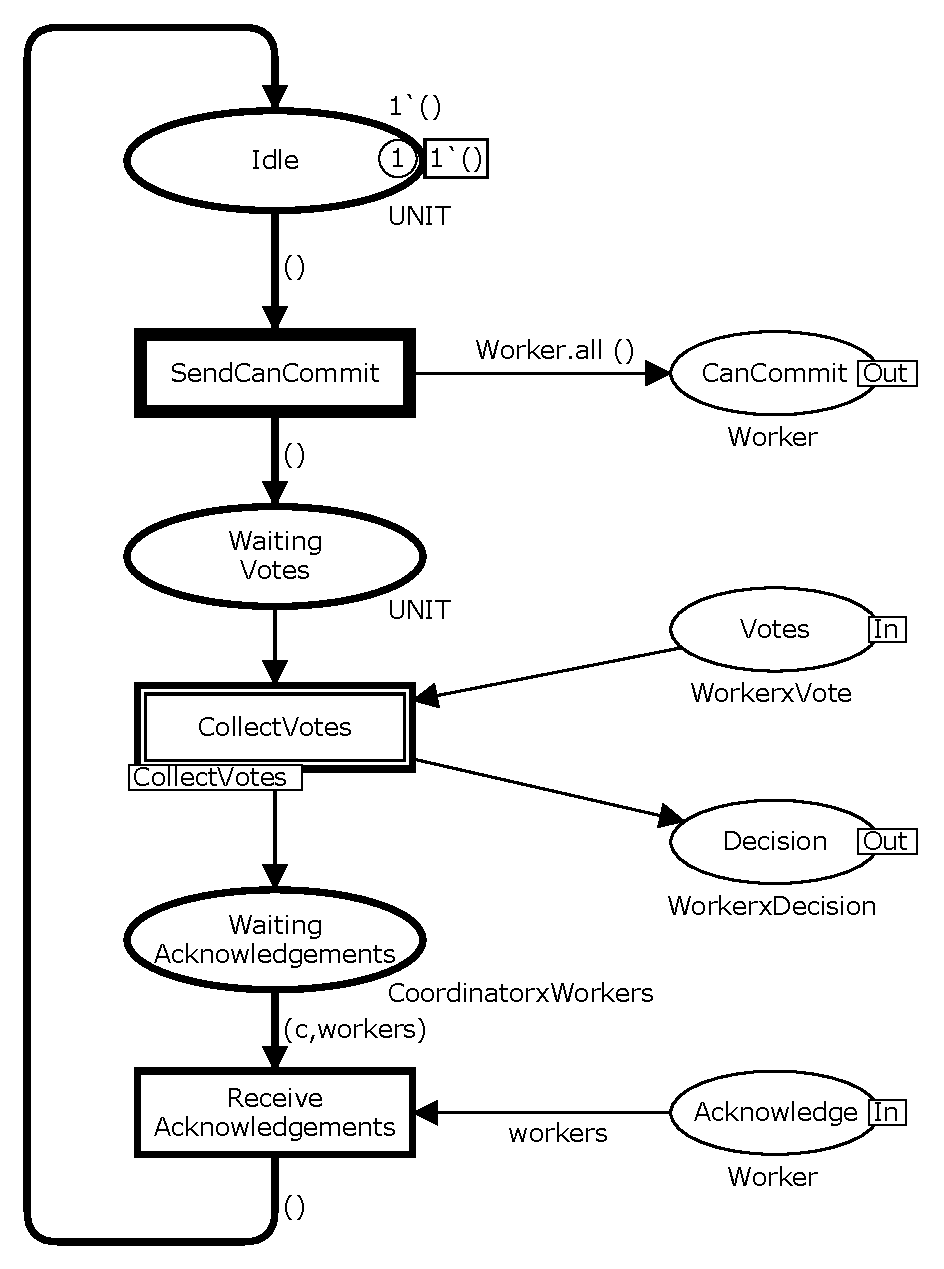
\includegraphics[scale=.45]{figures/Coordinator.eps}
\caption{The \figitem{Coordinator} module.}
\label{fig:coordinator}
\end{figure}



The places \figitem{Idle}, \figitem{WaitingVotes}, and
\figitem{WaitingAcknowledgement} are used to model the states of the
coordinator when executing the two-phase commit protocol. The places
\figitem{Idle} and \figitem{WaitingVotes} have the color set
\smlcode{UNIT} containing just a single value \smlcode{()} (denoted
unit). Initially, the coordinator is in an idle state as modeled by
the initial marking of place \figitem{Idle} which consists of a single
token with the color unit. In CPN ML this multi-set is written
\smlcode{1`()} specifying one (\smlcode{1}) occurrence of
(\smlcode{`}) the unit color (\smlcode{()}).  The number of tokens on
a place in the current marking is indicated with a small circle
positioned next to a place, and the detail of the color of the tokens
are provided in an associated text box. The indication of the current
marking of a place is omitted if currently the place contains no
tokens.

The transitions \figitem{SendCanCommit}, \figitem{CollectVotes}, and
\figitem{Receive\linebreak[4]Acknowledgements} model the
events/actions that cause the coordinator to change state. The
coordinator will first send a can commit message (transition
\figitem{SendCanCommit}) to each worker asking whether they can commit
the transaction. Then the coordinator will collect the votes from all
workers (substitution transition \figitem{CollectVotes}) and send a
decision to the workers that voted yes indicating whether the
transaction is to be committed or not. Finally, the coordinator will
receive an acknowledgment from each worker that voted yes, confirming
that they have received the decision (transition
\figitem{ReceiveAcknowledgements}).  It should be noted that
\figitem{CollectVotes} is a substitution transition which means that
the details of how the coordinator collects votes is modeled by the
associated \figitem{CollectVotes} submodule. This illustrates the
mixed use of ordinary and substitution transitions within a module. We
omit the details of \figitem{CollectVotes} in this paper.

% basic enabling and occurrences

In the current marking shown in Fig.~\ref{fig:coordinator} only the
transition \figitem{SendCanCommit} is enabled as indicated by the
thick border of that transition. The requirement for a transition to
be \concept{enabled} is determined from the \concept{arc expressions}
associated with the incoming arcs of the transition. In this case,
there is only a single incoming arc from place \figitem{Idle}
containing the expression \smlcode{()}. This expression specifies that
for \figitem{SendCanCommit} to be enabled, there must be at least one
\smlcode{()}-token present on \figitem{Idle}. When the
\figitem{SendCanCommit} transition \concept{occurs}, it will consume a
\smlcode{()}-token from place \smlcode{Idle} and it will produce
tokens on places connected to output arcs as determined by
\concept{evaluating} the arc expressions on output arcs. In this case,
the expression \smlcode{()} on the arc to \smlcode{WaitingVotes}
evaluates to a single \smlcode{()}-token. The expression
\smlcode{Worker.all()} is a call to the function \smlcode{Worker.all}
that takes a unit value (\smlcode{()}) as parameter and returns all
colors of the color set \smlcode{Worker}. This illustrates how complex
calculations (e.g., of multi-sets of tokens or involving tokens with
complex data values) can be encapsulated within function calls, and
how several tokens can be added/removed in a single step (transition
occurrence) without introducing intermediate states (markings).

\ignore{
This illustrates that arc expression may also make
use of function to calculate the tokens to be added (removed) from
places. In particular this means that complex data manipulation can be
performed without intruding intermediate steps in the model itself.
}

Figure~\ref{fig:sendcancommit} shows the marking of the surrounding
places of transition \figitem{SendCanCommit} after the occurrence of
\figitem{SendCanCommit}. It can be seen that the place
\figitem{CanCommit} contains two tokens (one of each worker in the
system) representing messages going to the two worker processes. The
coordinator has now entered a state in which it is waiting to collect
the votes from the worker processes.

\begin{figure}[b]
\centering
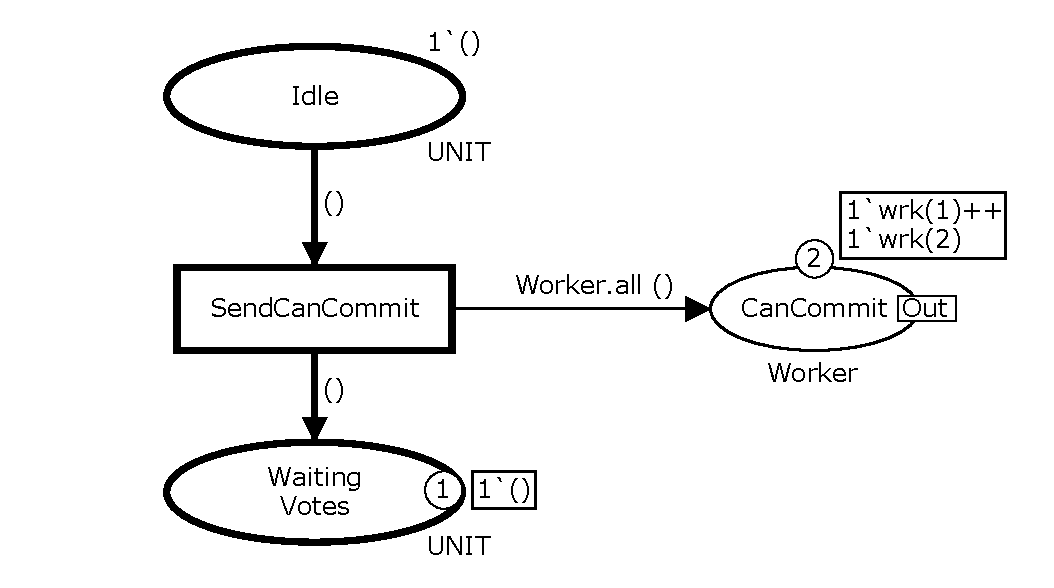
\includegraphics[scale=.45]{figures/SendCanCommit.eps}
\caption{Current marking after \figitem{SendCanCommit}.}
\label{fig:sendcancommit}
\end{figure}

% comparison to low-level nets


%\com{Maybe we could have shown
%  the corresponding fragment as a Place/Transition net? In this case we need more places - when we get to the worker we could also need to duplicate transition as per bindings}

% worker process - and binding and binding elements.

Figure~\ref{fig:worker} shows the \figitem{Worker} module which is the
submodule of the \figitem{Workers} substitution transition in
Fig.~\ref{fig:commit}. The places \figitem{CanCommit},
\figitem{Votes}, \figitem{Decision}, and \figitem{Acknowledge}
constitute the port places of this module and are linked to the
accordingly named socket places in Fig.~\ref{fig:commit}. The places
\figitem{Idle} and \figitem{WaitingDecision} model the two main states
of worker processes. Each of these places have the color set
\smlcode{Worker} and the idea is that when there is a token with color
\smlcode{wrk(i)} on, e.g., the place \figitem{Idle}, then this models
that the i'th worker is in state idle. This makes it possible to model
the state of all workers in a compact manner within a single module
without having to have a place for each worker or a module instance
for each worker. Initially, all workers are in the idle state as
represented by corresponding tokens on place \figitem{Idle} in the
initial marking. The transition \figitem{ReceiveCanCommit} models the
reception of can-commit messages from the coordinator and the sending
of a vote. The transition \figitem{ReceiveDecision} models the
reception of a decision message from the coordinator and the sending
of an acknowledgment.

\begin{figure}[]
\centering
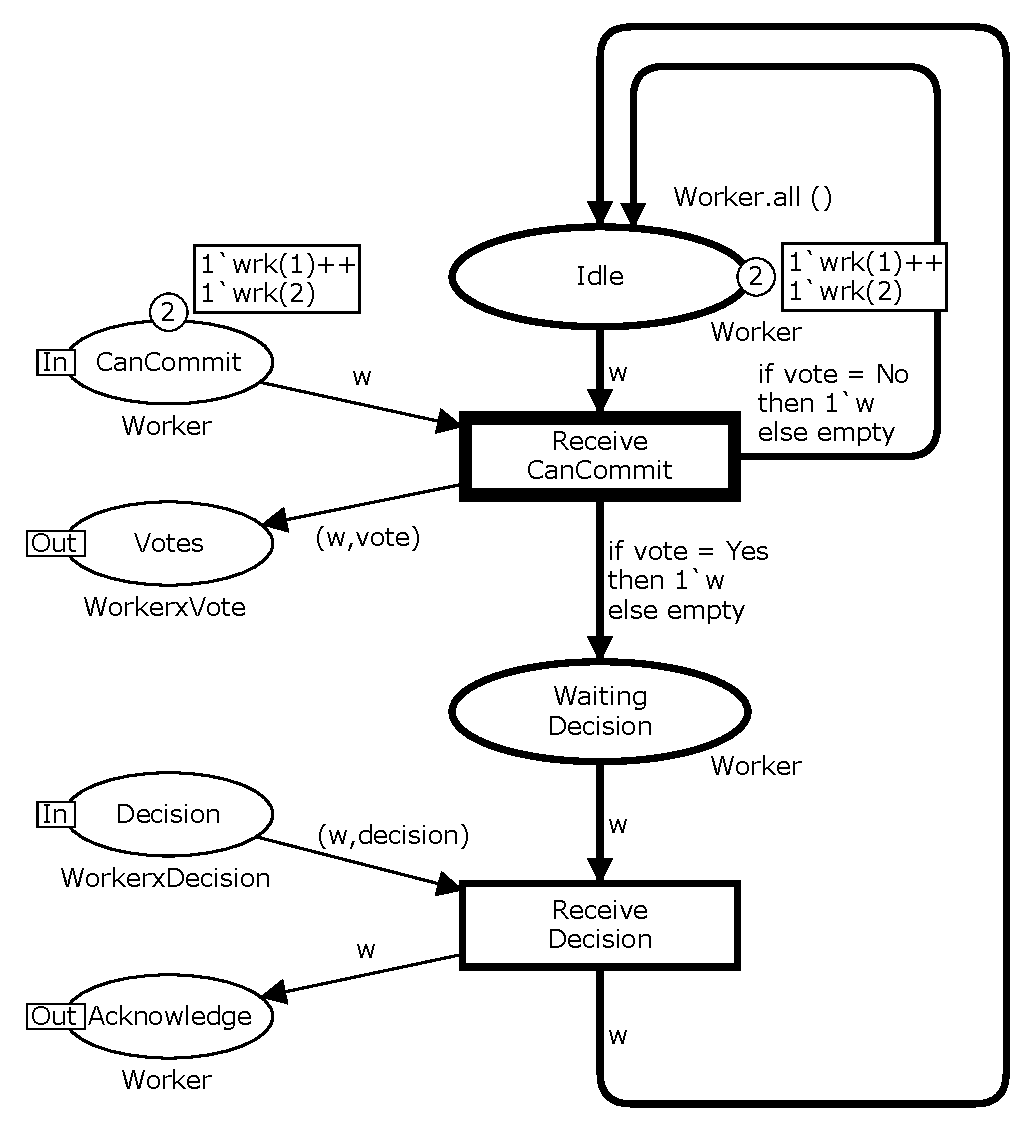
\includegraphics[scale=.45]{figures/Workers.eps}
\caption{The \figitem{Worker} module.}
\label{fig:worker}
\end{figure}

The current marking of place \figitem{CanCommit} in
Fig.~\ref{fig:worker} is \smlcode{1`wrk(1) ++ 1`wrk(2)} modeling a
marking where the coordinator has sent a can-commit message to each
worker. The thick border of transition \figitem{ReceiveCanCommit}
indicates that this transition is enabled in the current marking. The
arc expressions on the surrounding arcs of the
\figitem{ReceiveCanCommit} transition are more complex than the arc
expressions of the \figitem{SendCanCommit} transition in the
\figitem{Coordinator} module considered earlier in that they contain
the \concept{free variables} \smlcode{w} and \smlcode{vote} defined in
Fig.~\ref{fig:coloursets}. This means that in order to talk about the
enabling and occurrence of transition \figitem{ReceiveCanCommit}, we
need to bind (assign) values to these variables in order to evaluate
the input and output arc expressions. This is done by creating a
\concept{binding} which associates a value to each of the free
variables occurring in the arc expression of the transition. Bindings
can be considered different modes in which a transition may occur.  As
\smlcode{w} is of type \smlcode{Worker} and \smlcode{vote} is of type
\smlcode{Decision}, this gives the bindings listed in
Fig.~\ref{fig:bindings} reflecting that each of the two workers may
vote \smlcode{Yes} or \smlcode{No} to committing the transactions.

\begin{figure}[]
\centering
\begin{eqnarray*}
b_{1Y} & = & \langle \smlcode{w} = \smlcode{wrk(1)}, \smlcode{vote} = \smlcode{Yes} \rangle \\
b_{1N} & = & \langle \smlcode{w} = \smlcode{wrk(1)}, \smlcode{vote} = \smlcode{No} \rangle \\
b_{2Y} & = & \langle \smlcode{w} = \smlcode{wrk(2)}, \smlcode{vote} = \smlcode{Yes} \rangle \\
b_{2N} & = & \langle \smlcode{w} = \smlcode{wrk(2)}, \smlcode{vote} = \smlcode{No} \rangle
\end{eqnarray*}
\caption{Bindings of transition \figitem{ReceiveCanCommit}.}
\label{fig:bindings}
\end{figure}

A binding of a transition is enabled if evaluating each input arc
expression in the binding results in a multi-set of tokens which is a
subset of the multi-set of tokens present on the corresponding input
place. For an example, consider the binding $b_{1Y}$. Evaluating the
input arc expression \smlcode{w} on the input arc from \figitem{Idle}
results in the multi-set containing a single token with the color
\smlcode{wrk(1)} which is contained in the multi-set of tokens present
on place \figitem{Idle} in the marking depicted in
Fig.~\ref{fig:worker}. Similarly for the input arc expression on the
arc from place \figitem{CanCommit}. This means that binding $b_{1Y}$
is enabled and may occur. In fact, all four bindings listed in
Fig.~\ref{fig:bindings} is enabled in the marking shown in
Fig.~\ref{fig:worker}.

% ocurrence and more complicated evaluation

The tokens produced on output places when a transition occurs in an
enabled binding is determined by evaluating the output arc expressions
of the transition in the given binding. Consider again the binding
element $b_{1Y}$. The output arc expression \smlcode{(w,vote)}
evaluates to \smlcode{(wrk(1),Yes)} and this token will be added to
place \figitem{Votes} to inform the coordinator that worker one votes
yes to committing the transaction. The arc expression on the arc from
\figitem{ReceiveCanCommit} to \figitem{WaitingDecision} is an
if-then-else expression which in the binding $b_{1Y}$ evaluates to the
multi-set \smlcode{1`wrk(1)} which will be added to the tokens on
place \figitem{WaitingDecision}. The if-then-else expression on the
arc from \figitem{ReceiveCanCommit} to \figitem{Idle} evaluates to the
\smlcode{empty} multi-set and hence no tokens will be added to place
\figitem{Idle} in this case. Figure~\ref{fig:receivecancommit} shows
the marking resulting from an occurrence of the $b_{1Y}$ binding.

\begin{figure}[b]
\centering
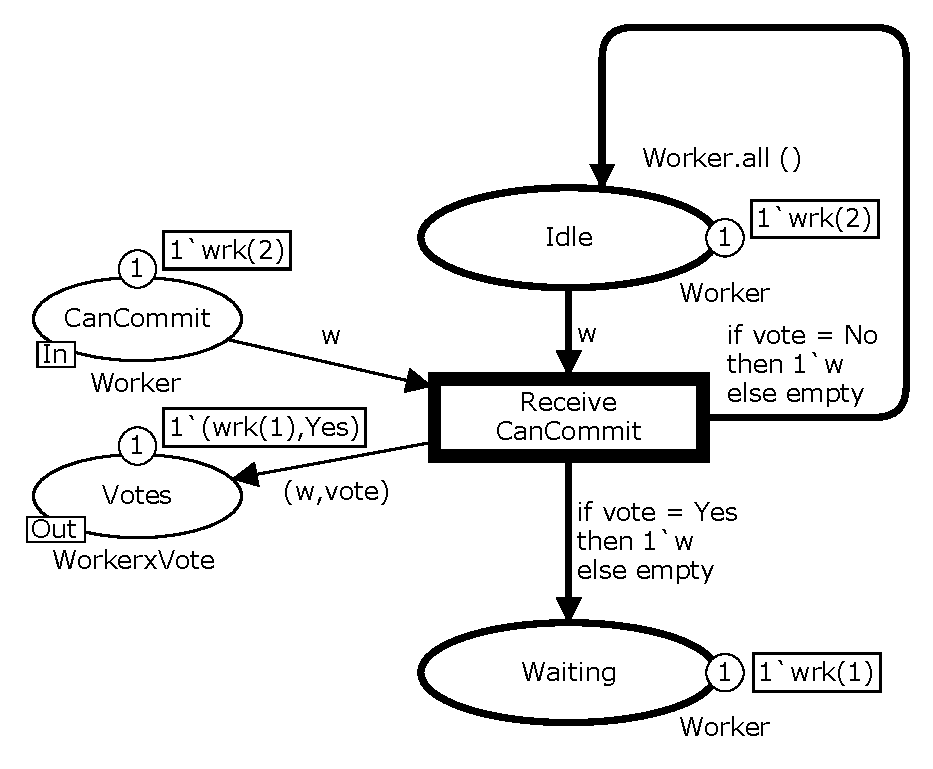
\includegraphics[scale=.45]{figures/ReceiveCanCommit.eps}
\caption{Current marking after \figitem{ReceiveCanCommit}.}
\label{fig:receivecancommit}
\end{figure}

The occurrence of the binding $b_{1N}$ representing that worker one
votes no would have the effect of removing a \smlcode{wrk(1)}-token
from \figitem{Idle}, adding a \smlcode{(wrk(1),No)}-token to
\figitem{Votes}, adding no tokens to place \figitem{WaitingDecision},
and adding a \smlcode{wrk(1)}-token to place \figitem{Idle}. This
models the fact that if a worker votes no to committing the
transaction, then it goes back to idle; whereas if it votes yes, then
it will go to waiting to be informed about whether the transaction is
to be committed or not.  As this is a distributed system a worker
cannot without exchanging messages know the vote of another worker.

% concurrency
All four bindings listed for transition \figitem{ReceiveCanCommit}
were enabled in the marking shown in Fig.~\ref{fig:worker}. Enabled
bindings may be \concept{concurrently enabled} if each binding can get
its required multi-set of tokens from each input place independently
of the other enabled bindings in the set. As an example, the two
bindings $b_{1Y}$ and $b_{2Y}$ are concurrently enabled since each
binding can get its token from the input places without sharing with
each other. This reflects that the workers are executing concurrently
and may simultaneously send a vote back to the coordinator. In
contrast, the two bindings $b_{1Y}$ and $b_{1N}$ are not concurrently
enabled. These two bindings are in \concept{conflict} because they
each need the single \smlcode{wrk(1)}-token on \figitem{Idle} (and in
fact also the single \smlcode{wrk(1)}-token on place
\figitem{CanCommit}). The notion of concurrency and conflict of binding
extends to bindings of different transitions. A fundamental property
of a set of concurrently enabled bindings that CPNs inherit from Petri
nets is that these can be executed in any interleaved order and the
resulting marking will be the same independently of the interleaved
execution considered.\\

% a few comments about other constructed in the language
 Above relatively simple arc expressions were used. In general, arc
 expressions can be any expression that can be written in Standard ML
 as long as they have types that matches the corresponding places. In
 particular, arc expressions may apply functions including
 higher-order functions. CPNs also includes a notion of time inspired
 by the work of van der Aalst \cite{X} that makes it possible to model
 the time taken by different activities. It is based on the
 introduction of a \concept{global model clock} that represents the
 current model time and on attaching \concept{time stamps} to tokens
 in addition to the token colors. The time stamp of a token specifies
 the earliest model time at which the token can be removed by the
 occurrence of a transition, and delay inscriptions on the transitions
 and arcs are used to determine the timestamps on tokens produced by
 transitions. During model execution, the global model clock is always
 advanced to the earliest next time at which a transition becomes
 enabled, and the model stays at the current model time until no more
 transitions are enabled. The time concept provides the foundation for
 conducting simulation-based performance analysis of CPN models. 

%i(see
% sidebar on Performance Analysis).



%\section{An Example CPN Model}

\begin{figure*}[t]
\centering
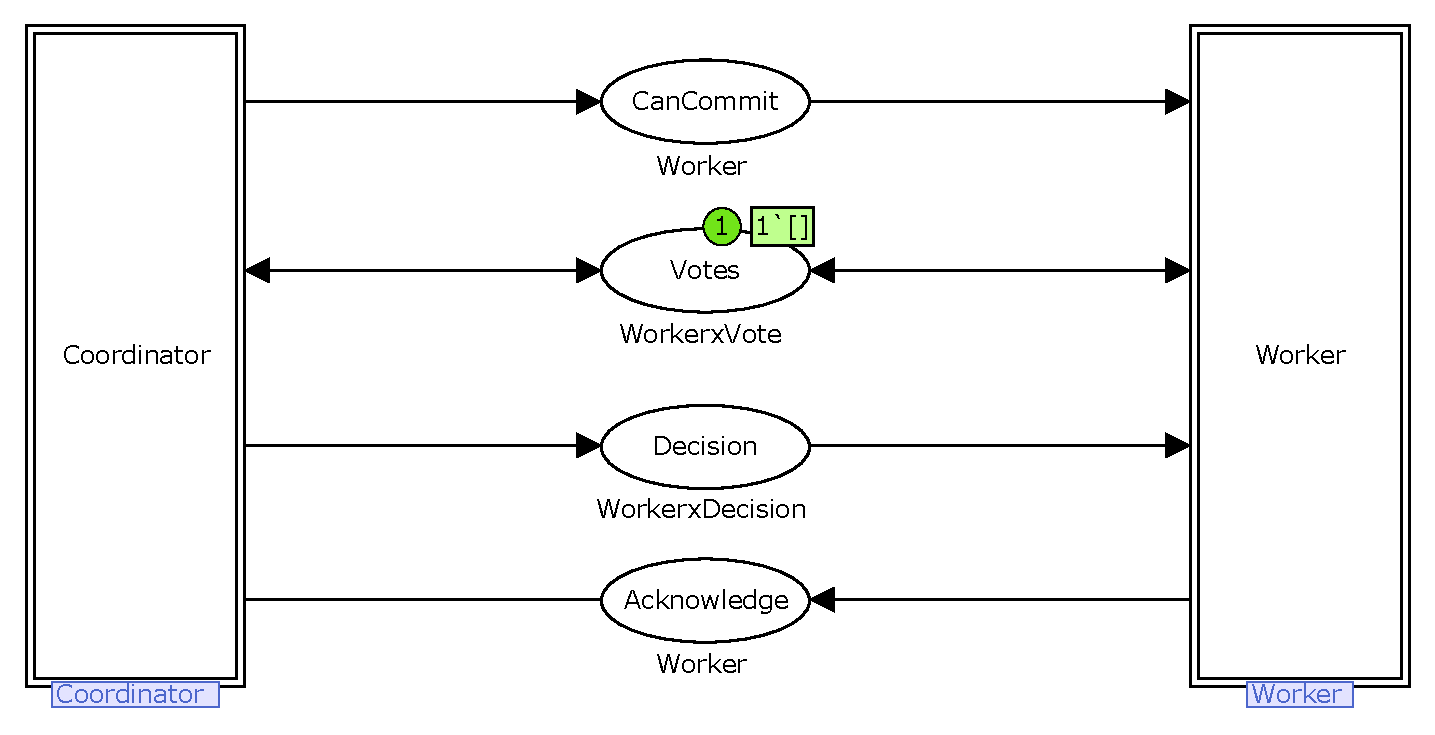
\includegraphics[width=15cm]{figures/Commit.eps}
\caption{The top-level Commit module of the CPN model.}
\end{figure*}

\begin{figure}[t]
\centering
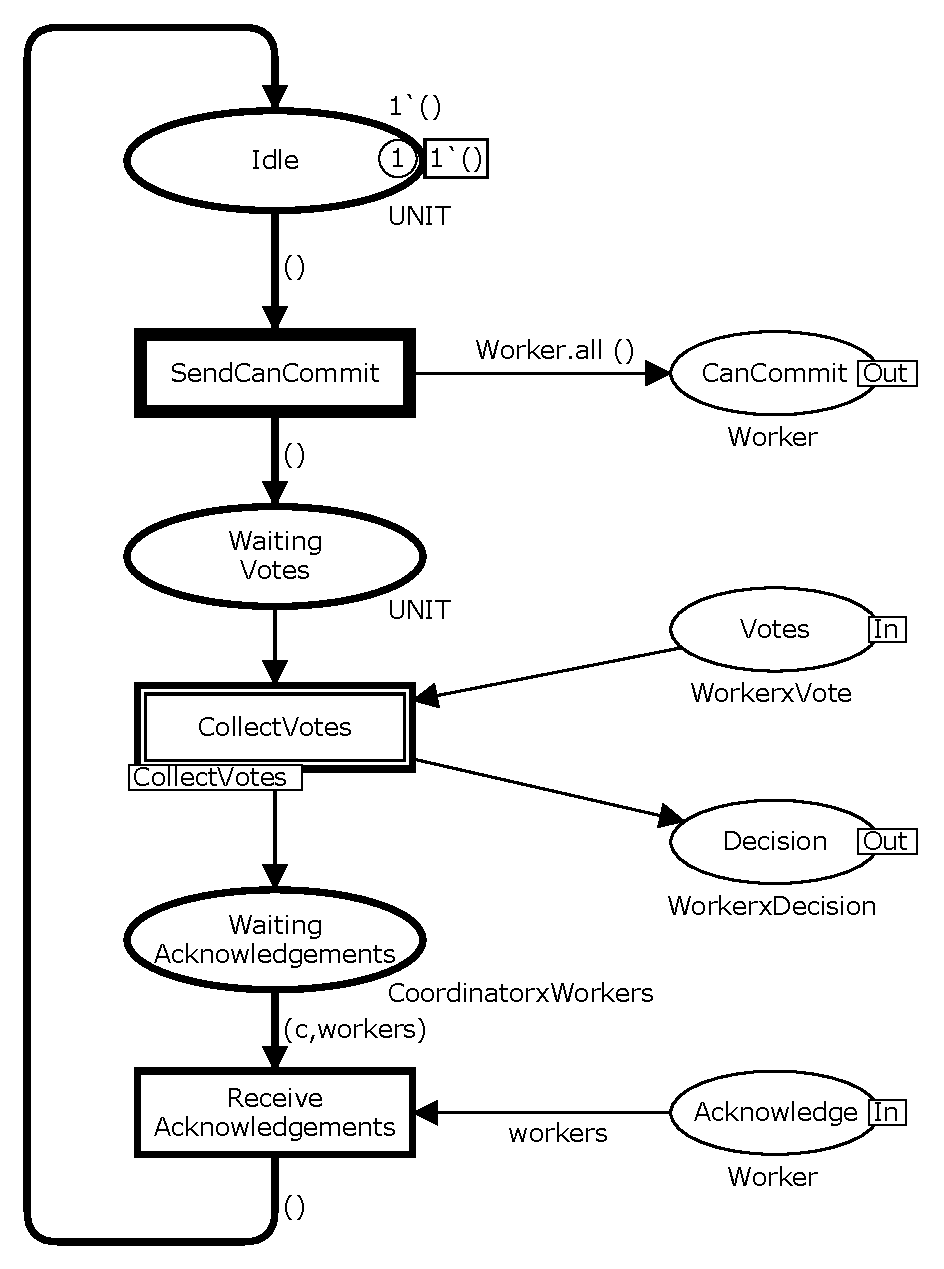
\includegraphics[width=\columnwidth]{figures/Coordinator.eps}
\caption{The Coordinator module.}
\end{figure}

\begin{figure}[t]
\centering
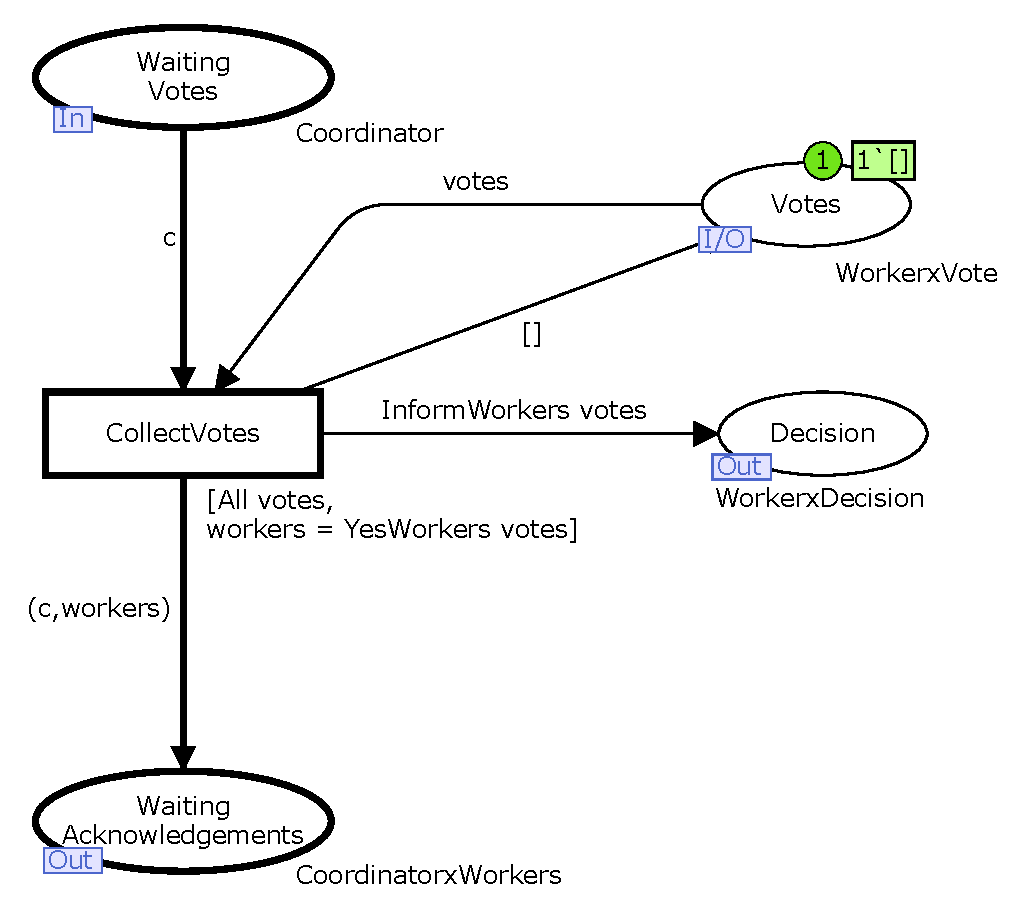
\includegraphics[width=\columnwidth]{figures/CollectVotes.eps}
\caption{The CollectVotes module.}
\end{figure}

\begin{figure}[t]
\centering
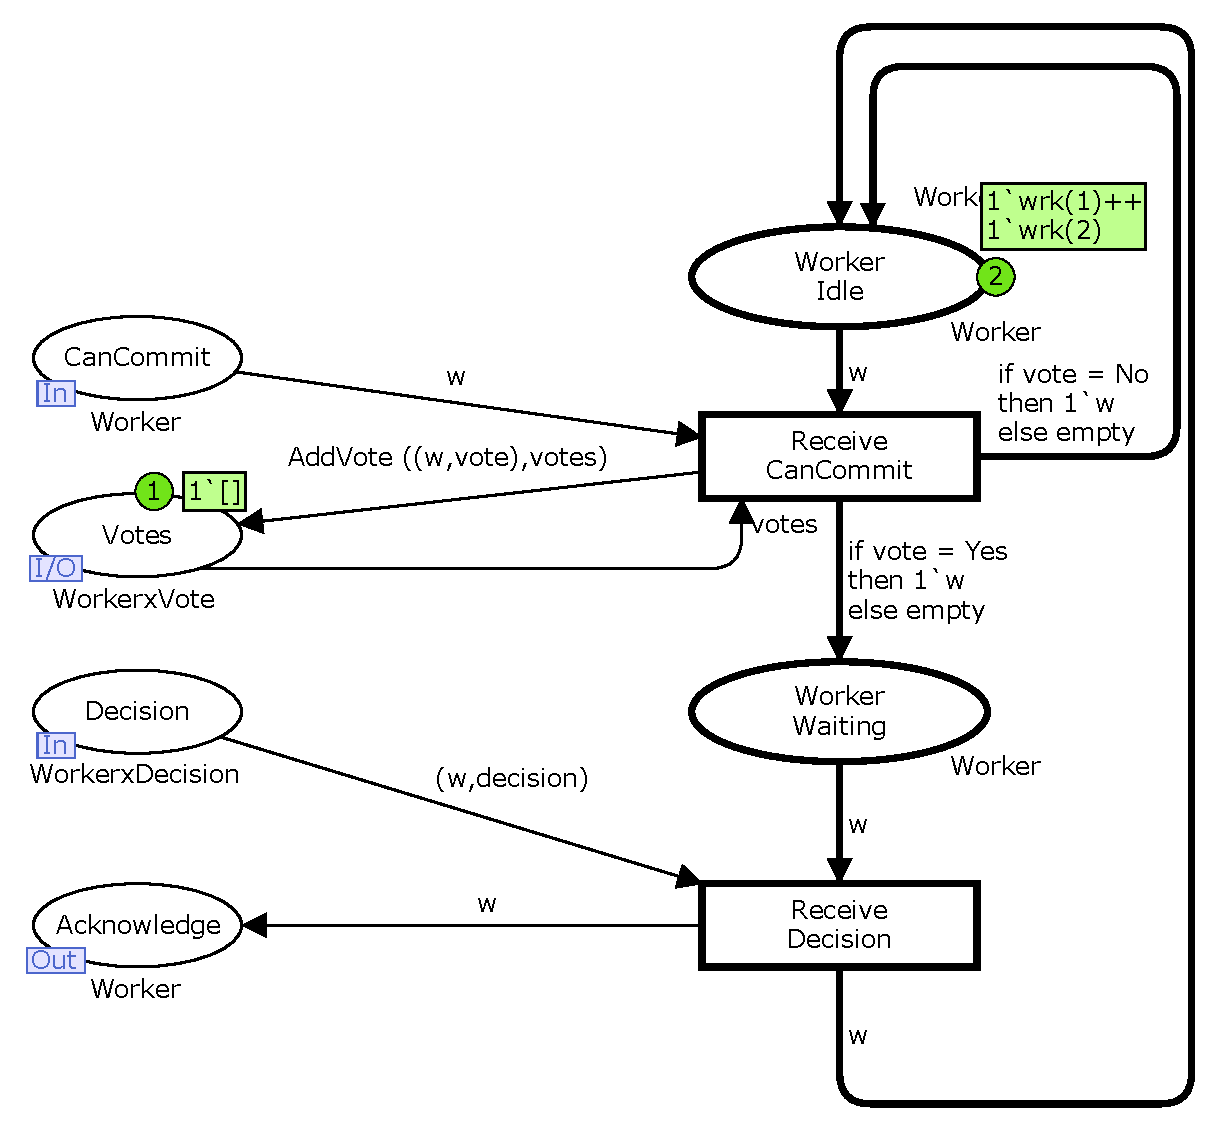
\includegraphics[width=\columnwidth]{figures/Worker.eps}
\caption{The Worker module.}
\end{figure}

\begin{figure}
\begin{verbatim}
colset INT = int;
var i : INT;

colset Coordinator = with c;
colset CoordinatorxInt = product Coordinator * INT;

colset Worker = index wrk with  1..2;
var w: Worker;

colset WorkerList = list Worker;
var workers : WorkerList;

colset CoordinatorxWorkers = product Coordinator * WorkerList;

colset Vote = with Yes | No;
var vote : Vote;

colset WorkerxVotes = product Worker * Vote;
colset WorkerxVote = list WorkerxVotes;
var votes : WorkerxVote;

colset Decision = with abort | commit;
var decision : Decision;

colset WorkerxDecision = product Worker * Decision;
\end{verbatim}
\caption{Colour sets and variable declarations.}
\end{figure}

\begin{figure}
\begin{verbatim}
val Workers = Worker.all();

fun AddVote ((w,vote),votes) = 
    sort_ms WorkerxVotes.lt ((w,vote)::votes);

fun YesWorkers votes = 
    List.map (fn (w,_) => w) 
      (List.filter (fn (w,Yes) => true 
                     | (w,No) => false) votes);

fun InformWorkers votes = 
    if (List.all (fn (_,Yes) => true 
                   | _ => false) votes)
                                            
    then List.map (fn w => (w,commit)) (YesWorkers votes)
    else List.map (fn w => (w,abort)) (YesWorkers votes);

fun All votes = List.length votes = List.length (Worker.all());
\end{verbatim}
\caption{Values and function definitions.}
\end{figure}


\section{Timed CPNs}

\section{Analysis and Validation}

\section{Tools and Applications}

The construction and analysis of CPN models have been supported by two
generations of graphical software tools: Design/CPN \cite{tacas97} and
CPN Tools \cite{cpn2003}. These tools have been instrumental to the
success of CPNs as they have enabled the practical use in a broad
range of domains such as distributed software systems, communication
protocols, embedded systems, and process- and workflow modeling. A
comprehensive list containing more than hundred papers describing
practical applications and domains is available \cite{cpnuse}.

% Design/CPN and CPN Tools - history
The Design/CPN tool \cite{tacas97} was created at Meta Software,
Cambridge, Massachusetts, USA starting in 1988. The main architects
behind the tool were Jensen, Shapiro and Huber, and the implementation
was made together with an international group of people. The first
version of Design/CPN supported modeling, syntax cheek and interactive
simulation. The introduction of hierarchical CPNs supported by the
Design/CPN tool made a dramatic change to the practical use of Petri
nets. The new modeling language and its tool support were general and
powerful enough to eliminate the need of making ad-hoc extensions as
discussed in the introduction of this paper. A common platform for
practical modeling had been established and this was used by most
Petri net practitioners. The use of the platform was supported by a
three volume monograph on Colored Petri Nets published by Jensen in
1992-1997 \cite{jensen:cpnvols}.

Starting from year 2000 a second generation of tool support, called
CPN Tools, was designed and implemented at Aarhus University. The main
architects behind the new tool were Jensen, Christensen, and
Westergaard \cite{cpn2003}.  It was based on empirical studies of the
use of Design/CPN and much easier and efficient to use when
constructing CPN models. In 2010, CPN Tools had $10,000$ licenses in 150
countries. At that time the development and maintenance of the tool
set were transferred to the group of van der Aalst at the Technical
University of Eindhoven \cite{cpntoolsweb}. New updates with improved
functionality are made at a regular basis.

% Illustration of CPN Tools.
CPN Tools supports the editing and construction of CPN models,
interactive and automatic simulation, state space-based model checking
(see Sidebar~II), and simulation-based performance analysis (see
Sidebar~III). CPN Tools is based on a much faster simulation engine
developed by Haagh, Hansen, and Mortensen \cite{mortensen:01}. With
this simulation engine, many models run more than thousand times
faster compared to Design/CPN allowing complex automatic simulations
to be executed within seconds instead of hours. The state space
methods supported by CPN Tools have been developed by Christensen,
Kristensen, Westergaard, Evangelista, and Mailund
\cite{sweep,asap}. The support for performance
analysis is based on the work of Wells and Lindstr\o{}m
\cite{performance1}.

\begin{figure*}[t]
\centering
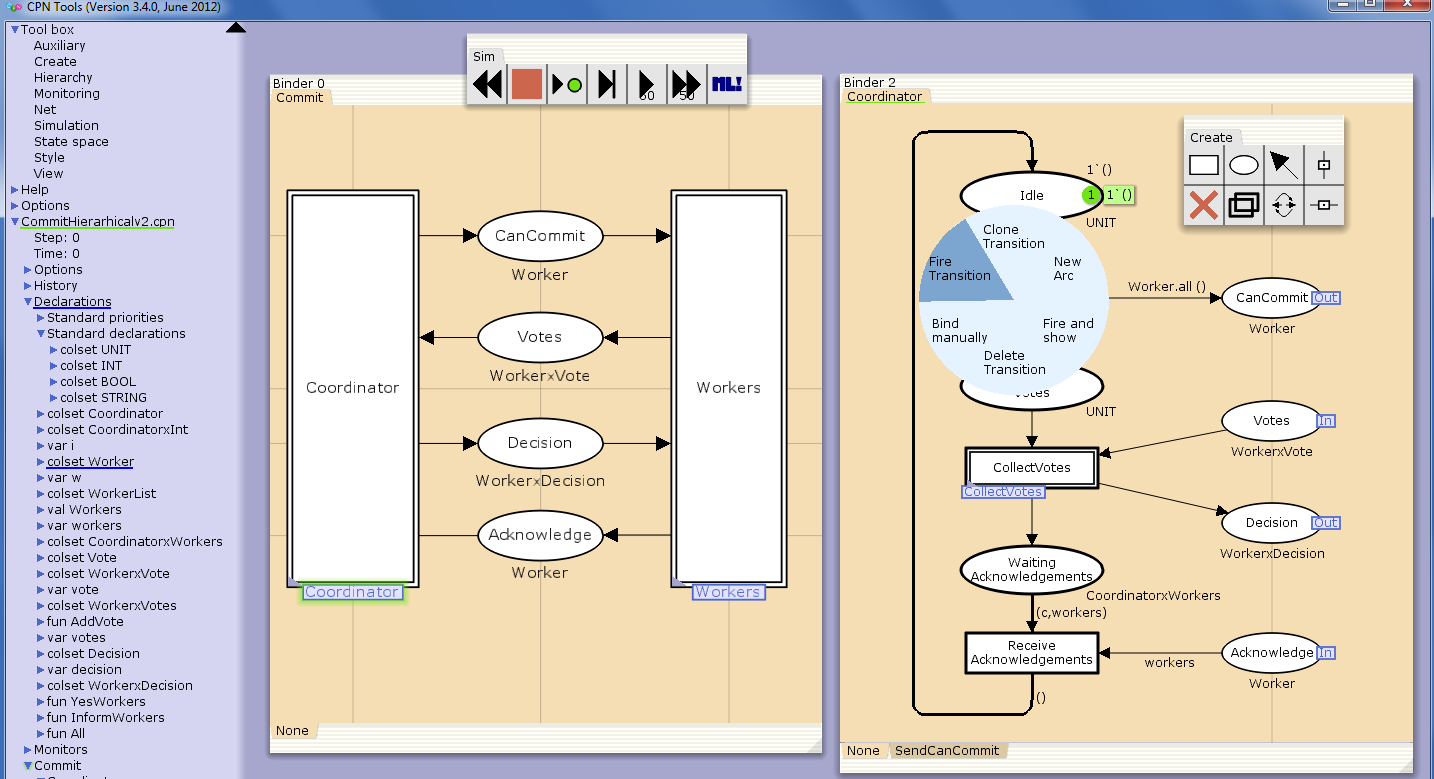
\includegraphics[scale=.37]{figures/cpntools.png}
\caption{The two-phase commit CPN model in CPN Tools}
\label{fig:cpntools}
\end{figure*}

Figure~\ref{fig:cpntools} provides a screen-shot of CPN Tools with the
CPN model considered in this paper. The user of CPN Tools works
directly with the graphical representation of the CPN model. The
graphical user interface of CPN Tools has no conventional menu bars
and pull-down menus, but is based on interaction techniques, such as
\concept{tool palettes} and \concept{marking menus}. The rectangular
area to the left is an \concept{index}. It includes the \figitem{Tool
  box}, which is available for the user to manipulate the declarations
and modules that constitute the CPN model. The \figitem{Tool box}
includes tools for creating, copying, and cloning the basic elements
of CPNs. It also contains a wide selection of tools to manipulate the
graphical layout and the appearance of the objects in the CPN
model. The latter set of tools is very important in order to be able
to create readable and graphically appealing CPN models. The remaining
part of the screen is the \concept{workspace}, which in this case
contains two \concept{binders} (the rectangular windows) and a
circular pop-up menu.\rdc{Each binder may hold a number of items which can
be accessed by clicking the tabs at the top of the binder (only one
item is visible at a time).} In the example shown, there are two
binders with one item each. One binder (left) containing the
\figitem{Commit} module and one binder (right) containing the
\figitem{Coordinator} module. In addition, two tool palettes are
shown: one (\figitem{Sim}) containing the tools that can be used for
simulation of the model, and another (\figitem{Create}) containing the
tools for creating CPN model elements.\rdc{Items can be dragged from the
index to the binders, and from one binder to another binder.} A
circular marking menu has been popped up on top of a transition in the
binder to the right. Marking menus are contextual menus that make it
possible to select among the operations possible on a given object. In
this case, the marking menu gives the operations that can be performed
on a transition.




\ignore{

 contains three
modules named \figitem{Protocol}, \figitem{Sender}, and
\figitem{Receiver}, while another binder contains a single module,
named \figitem{Network}, together with the declaration of the colour
set \smlcode{NOxDATA}. The two remaining binders contain four
different tool palettes to \figitem{Create} elements, change their
\figitem{Style}, perform \figitem{Simulations}, and construct
\figitem{State spaces}.

There are two kinds of binders. One kind contains the
elements of the CPN model, i.e., the modules and declarations. The
other kind contains the tools which the user applies to construct and
manipulate CPN models. The tools in a tool palette can be picked up
with the mouse cursor and applied. In the example shown, one binder
contains three modules named \figitem{Protocol}, \figitem{Sender}, and
\figitem{Receiver}, while another binder contains a single module,
named \figitem{Network}, together with the declaration of the color
set \smlcode{NOxDATA}. The two remaining binders contain four
different tool palettes to \figitem{Create} elements, change their
\figitem{Style}, perform \figitem{Simulations}, and construct
\figitem{State spaces}.
}

% syntax check and code generation and simulation

CPN Tools performs syntax and type checking, and contextual error
messages are provided to the user. The syntax check and code generation are
incremental and are performed in parallel with editing. This means
that it is possible to execute parts of a CPN model even if the model
is not complete, and that when parts of a CPN model are modified, a
syntax check and code generation are performed only on the elements
that depend on the parts that were modified. CPN Tools supports two
types of simulation: interactive and automatic. In an interactive
simulation, the user is in complete control and determines the
individual steps in the simulation, by selecting between the enabled
events in the current state. CPN Tools shows the effect of executing a
selected step in the graphical representation of the CPN model. In an
automatic simulation the user specifies the number of steps that are
to be executed and/or sets a number of stop criteria and
breakpoints. The simulator then automatically executes the model
without user interaction by making random choices between the enabled
events in the states encountered. Only the resulting state is shown in
the GUI but information about the executed steps can be collected in
various ways. CPN Tools also includes support for domain-specific
graphical feedback from simulations developed by Westergaard and
Lassen \cite{britney}.

\ignore{
  The
simulator of CPN Tools exploits a number of advanced data structures
for efficient simulation of large hierarchical CPN models. The
simulator exploits the locality property of Petri nets to ensure that
the number of steps executed per second in a simulation is independent
of the size of the CPN model. This guarantees that simulation scales
to large CPN models.
}






\bibliographystyle{abbrv}
\bibliography{sigproc}  % sigproc.bib is the name of the Bibliography in this case
\end{document}
